\documentclass[a4paper,12pt]{article} 


\usepackage[T2A]{fontenc}			% кодировка
\usepackage[utf8]{inputenc}			% кодировка исходного текста
\usepackage[english,russian]{babel}	% локализация и переносы


% Математика
\usepackage{amsmath,amsfonts,amssymb,amsthm,mathtools} 

\usepackage{gensymb}	
\usepackage{wasysym}

% Картинки
\usepackage{graphicx}
\graphicspath{{images/}}

%Заговолок
\usepackage[left=2cm,right=2cm,
    top=2cm,bottom=2cm,bindingoffset=0cm]{geometry}

\usepackage{titling}


\author{Петров Артём Антонович, группа 721}
\title{Лабораторная работа № 3.2.5 "Вынужденные колебания в электрическом контуре"}
\date{\today}

\begin{document} % начало документа

\begin{minipage}[t][5cm]{\textwidth}
\maketitle
\end{minipage}


\textbf{Цель работы:} 
\bigskip


\subsection*{Экспериментальная установка}
\bigskip


\begin{figure}[ht]
\centering
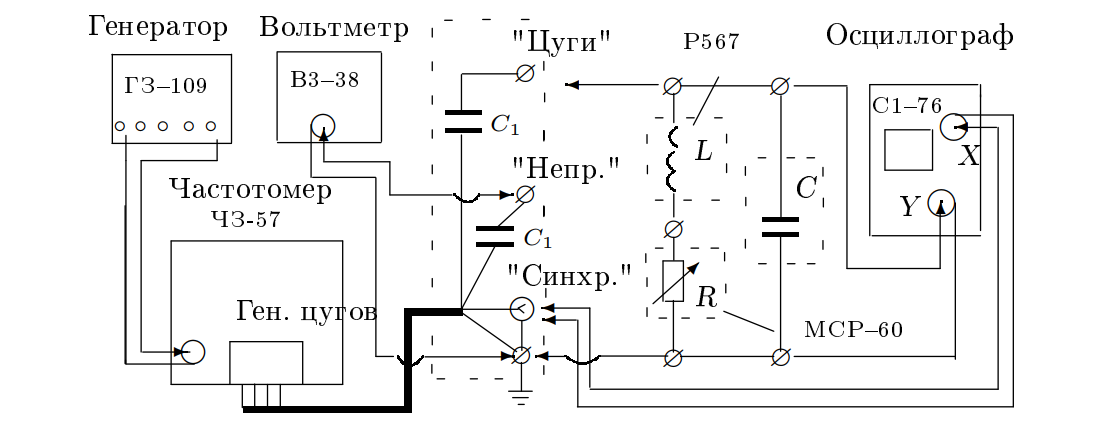
\includegraphics[width=150mm]{scheme.png}
\caption{Схема установки. (Исследуемый R-L-C контур и измерительные приборы)}\label{scheme.png}
\end{figure}

Параметры установки: $ C = (0.1 \pm 1\%)\mu F, L = (0.1\pm0.1\%)Hn $ .

\bigskip

\subsection*{Ход работы}
\bigskip

Были получены АЧХ в резонансе для разных значений R ((\ref{tbale1}),(\ref{graph})). 

\begin{figure}[h!]
\centering
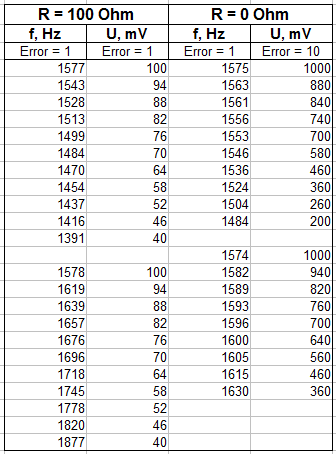
\includegraphics[width=70mm]{table1.png}
\caption{АЧХ колебательного контура в резонансе для двух разных значений R.}\label{tbale1}
\end{figure}

\begin{figure}[h!]
\centering
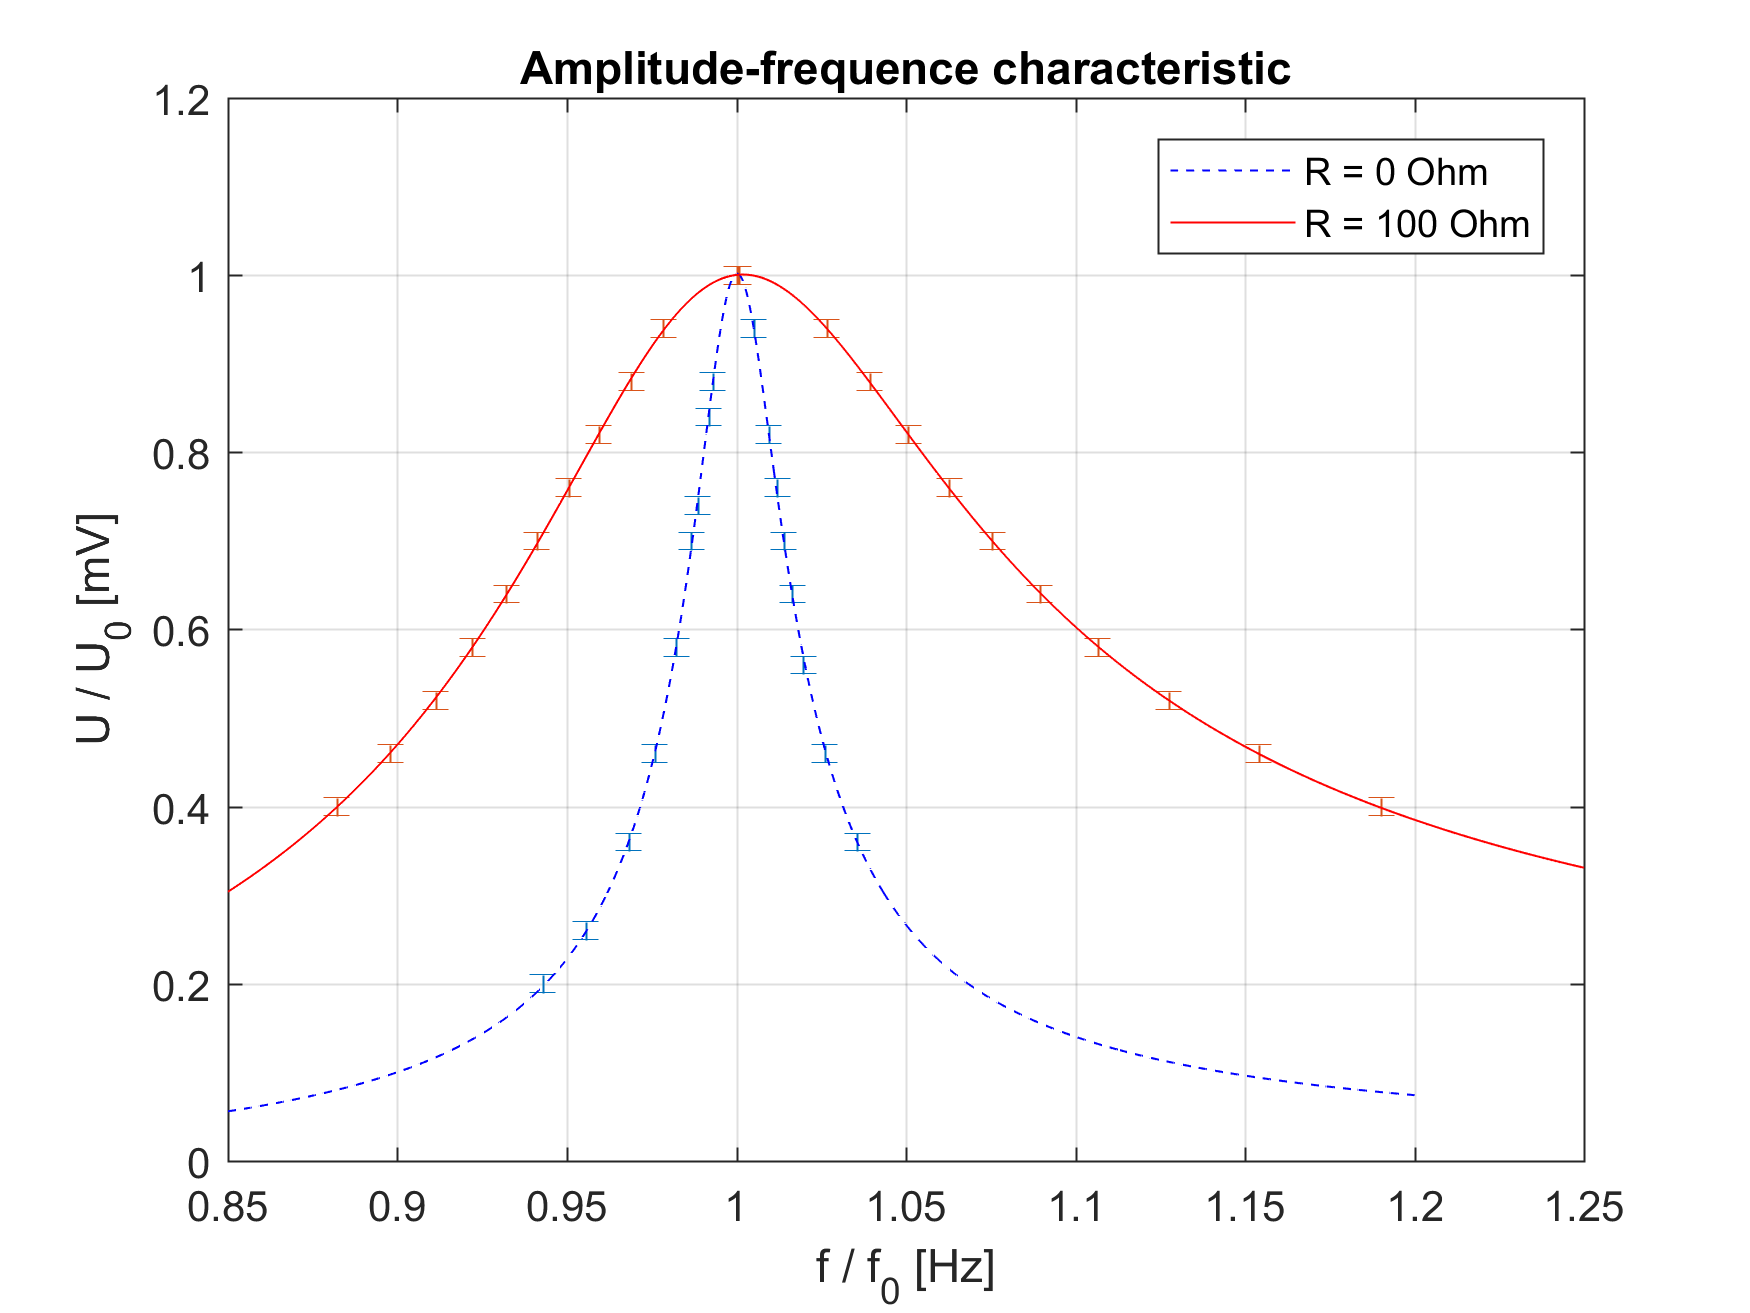
\includegraphics[width=150mm]{Plot.png}
\caption{АЧХ колебательного контура в резонансе для двух разных значений R.}\label{graph}
\end{figure}

По этим данным были рассчитаны значения добротности: 

$Q_{R=0\Omega} = (38\pm3),     Q_{R=100\Omega} = (7.6\pm1.1)$.

\medskip

Далее были получены зависимости амплитуды колебаний напряжения от номера колебания при их нарастании и затухании ((\ref{tbaleA0)}) и (\ref{tbaleA100)})).

По этим данным были рассчитаны значения добротности: 

При возрастании: $Q_{R=0\Omega} = (33\pm5),    Q_{R=100\Omega} = (8.7\pm0.7)$.

При затухании: $Q_{R=0\Omega} = (39\pm3),    Q_{R=100\Omega} = (7.7\pm0.6)$.

\begin{figure}[ht]
\centering
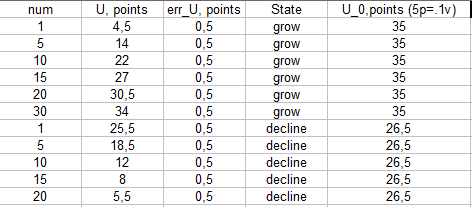
\includegraphics[width=90mm]{tableA0.png}
\caption{Амплитуды колебаний при возрастании и убывании сигнала для R=0Ом}\label{tbaleA0)}
\end{figure}


\begin{figure}[ht]
\centering
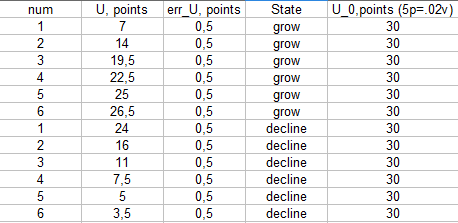
\includegraphics[width=90mm]{tableA100.png}
\caption{Амплитуды колебаний при возрастании и убывании сигнала для R=100Ом}\label{tbaleA100)}
\end{figure}
\bigskip

Также значение добротности было получено из теоретических соображений (по формуле $Q = \frac{1}{R}\sqrt{\frac{L}{C}}$) : 

$Q_{R=0\Omega} = 42.6\pm0.4),     Q_{R=100\Omega} = (8.1\pm0.1)$.


\bigskip

\newpage
.
\newpage
\subsection*{Итог}
\bigskip
 
 В данной работе был проанализирован процесс возникновения, и затухания вынужденных колебаний. Также было показано, что значение добротности, рассчитанное различными методами совпадает в пределах погрешностей, что показывает работоспособность применяемой модели вынужденных колебаний.
\end{document} % конец документа